\chapter{Раздел по охране труда и экологии}
\section{Анализ опасных и вредных факторов при разработке программного обеспечения и мероприятия по их устранению}

Разработка программного обеспечения требует длительного взаимодействия с вычислительными системами. Работа с персональными электронно-вычислительными машинами связана с рядом вредных и опасных факторов, таких как статическое электричество, рентгеновское излучение, электромагнитные поля, блики и отраженный свет, ультрафиолетовое излучение, мерцание изображения. При длительном воздействии на организм эти факторы негативно влияют на здоровье человека.

\subsection{Микроклимат}
Работа как программиста, так и пользователя относится к категории 1а, поскольку не предполагает больших физических усилий. Поэтому оптимальные нормы микроклимата для рабочего помещения программиста определяются табл. \ref{tab:microclimate} (СанПиН 2.2.2/2.4.1340-03).

\begin{table}[ht]
  \center
  \caption{Оптимальные нормы микроклимата}
  \begin{tabular}{|l|c|c|c|}
  \hline
  \multicolumn{1}{|p{0.15\textwidth}|}{}
  & \multicolumn{1}{|p{0.24\textwidth}|}{\centering Температура воздуха, $^\circ\mbox{C}$}
  & \multicolumn{1}{|p{0.31\textwidth}|}{\centering Относительная влажность воздуха, \%}
  & \multicolumn{1}{|p{0.2\textwidth}|}{\centering Скорость движения воздуха, м/с} \\
  \hline                       
  Холодный  & 22-24   & 40-60    & 0.1  \\ 
  \hline
  Теплый    & 23-25   & 40-60    & 0.1  \\ 
  \hline
  \end{tabular}
  \label{tab:microclimate}
\end{table}

Вредным фактором при работе с ЭВМ является также запыленность помещения. Этот фактор усугубляется влиянием на частицы пыли электростатических полей персональных компьютеров.

Для устранения несоответствия параметров указанным нормам проектом предусмотрено использование системы кондиционирования как наиболее эффективного и автоматически функционирующего средства. 

Нормы СанПиН 2.2.4.1294-03 «Санитарно-гигиенические нормы допустимых уровней ионизации воздуха» определяют уровни положительных и отрицательных ионов в воздухе (табл. \ref{tab:ionLevelInAir}):

\begin{table}[ht]
  \center
  \caption{Уровни ионизации воздуха помещений при работе на ВДТ и ПЭВМ}
  \begin{tabular}{|l|c|c|}
  \hline
  \multicolumn{1}{|p{0.4\textwidth}|}{\centering \multirow{2}{*}{Уровни}}
  & \multicolumn{2}{|p{0.4\textwidth}|}{\centering Число ионов в 1 $\text{см}^3$ воздуха} \\
  \cline{2-3} & \multicolumn{1}{|p{0.2\textwidth}|}{\centering $n^{+}$} & \multicolumn{1}{|p{0.2\textwidth}|}{\centering $n^{-}$} \\  
  \hline
  Минимально необходимые &  400 &  600 \\
  \hline
  Оптимальные		     &	1500-3000 & 3000-5000 \\
  \hline
  Предельно допустимые   & 50000 & 50000 \\
  \hline
  \end{tabular}
  \label{tab:ionLevelInAir}
\end{table}

Для обеспечения требуемых уровней предусмотрено использование системы ионизации Сапфир-4А.

Концентрация вредных химических веществ в помещениях с ПЭВМ не должна превышать «ПДК загрязняющих веществ в атмосферном воздухе населенных мест» ГН~2.1.6.789-99. Для выполнения указанных требований предусмотрено применение фильтров из активированного угля.


\subsection{Шум и вибрации}
Уровень шума на рабочем месте программиста не должен превышать 50~дБА, а уровень вибрации не должен превышать допустимых норм вибрации. СанПиН~2.2.2.542-96 устанавливает следующие нормы на вибрацию (табл. \ref{tab:noizeLevel}).

\begin{table}[ht]
  \center
  \caption{Допустимые нормы вибрации на рабочих местах с ВДТ и ПЭВМ}
  \begin{tabular}{|c|c|c|}
  \hline
  \multicolumn{1}{|c|}{\multirow{2}{0.4\textwidth}{\centering Среднегеометрические частоты октавных полос, Гц}}
  & \multicolumn{2}{|p{0.4\textwidth}|}{\centering Допустимые значения по виброскорости} \\
  \cline{2-3} & \multicolumn{1}{|p{0.2\textwidth}|}{\centering м/с} & \multicolumn{1}{|p{0.2\textwidth}|}{\centering дБ} \\  
  \hline
  2 & $4.5 \times 10$ & 79 \\
  \hline
  4 & $2.2 \times 10$ & 73 \\
  \hline
  8 & $1.1 \times 10$ & 67 \\
  \hline
  16 & $1.1 \times 10$ & 67 \\
  \hline
  31.5 & $1.1 \times 10$ & 67 \\
  \hline
  63 & $1.1 \times 10$ & 67 \\
  \hline
  \multicolumn{1}{|p{0.4\textwidth}|}{\centering Корректированные значения и их уровни в дБ} & \multirow{2}{*}{$2.0 \times 10$} & \multirow{2}{*}{72} \\
  \hline
  \end{tabular}
  \label{tab:noizeLevel}
\end{table}

При разработке программного обеспечения внутренними источниками шума являются вентиляторы, а также принтеры и другие периферийные устройства ЭВМ. 

Внешние источники шума – прежде всего, шум с улицы и из соседних помещений. Постоянные внешние источники шума, превышающего нормы, отсутствуют.

Для устранения превышения нормы проектом предусмотрено применение звукопоглощающих материалов для облицовки стен и потолка помещения, в котором осуществляется работа с вычислительной техникой.

\subsection{Освещение}
Наиболее важным условием эффективной работы программистов и пользователей является соблюдение оптимальных параметров системы освещения в рабочих помещениях.

Естественное освещение осуществляется через светопроемы, ориентированные в основном на север и северо-восток (для исключения попадания прямых солнечных лучей на экраны компьютеров) и обеспечивает коэффициент естественной освещенности (КЕО) не ниже 1.5\%.

В качестве искусственного освещения проектом предусмотрено использование системы общего равномерного освещения. В соответствии с СанПиН~2.2.2/2.4.1340-03  освещенность на поверхности рабочего стола находится в пределах 300-500~лк. Разрешается использование светильников местного освещения для работы с документами (при этом светильники не должны создавать блики на поверхности экрана).

Правильное расположение рабочих мест относительно источников освещения, отсутствие зеркальных поверхностей и использование матовых материалов ограничивает прямую (от источников освещения) и отраженную (от рабочих поверхностей) блескость. При этом яркость светящихся поверхностей не превышает 200 $\frac{\text{кд}}{\text{м}^2}$, яркость бликов на экране ПЭВМ не превышает 40 $\frac{\text{кд}}{\text{м}^2}$ и яркость потолка не превышает 200 $\frac{\text{кд}}{\text{м}^2}$.

В соответствии с СанПиН~2.2.2/2.4.1340-03  проектом предусмотрено использование люминесцентных ламп типа ЛБ в качестве источников света при искусственном освещении. В светильниках местного освещения допускается применение ламп накаливания.

Применение газоразрядных ламп в светильниках общего и местного освещения обеспечивает коэффициент пульсации не более 5\%.

Таким образом, проектом обеспечиваются оптимальные условия освещения рабочего помещения.

\subsection{Рентгеновское излучение}
В соответствии с СанПиН~2.2.2/2.4.1340-03, проектом предусмотрено использование ПЭВМ, конструкция которых обеспечивает мощность экспозиционной дозы рентгеновского излучения в любой точке на расстоянии 0.05 м от экрана и корпуса монитора не более 0.1 $\frac{\text{мбэр}}{\text{ч}}$ (100 $\frac{\text{мкР}}{\text{ч}}$). Результаты сравнения норм излучения приведены в табл. \ref{tab:rentgenNorm}.

\begin{table}[ht]
  \center
  \caption{Сравнение норм рентгеновского излучения в различных стандартах}
  \begin{tabular}{|l|c|c|c|}
  \hline
  \multicolumn{1}{|p{0.3\textwidth}|}{}
  & \multicolumn{1}{|p{0.3\textwidth}|}{\centering Допустимое значение, $\frac{\text{мкР}}{\text{ч}}$ не более} \\
  \hline
  СанПиН 2.2.2/2.4.1340-03 & 100 \\
  \hline
  TCO-99                   & 500 \\
  \hline
  MPR II                   & 500 \\
  \hline
  \end{tabular}
  \label{tab:rentgenNorm}
\end{table}

Как видно из табл.~\ref{tab:rentgenNorm}, стандарты MPR~II и TCO-99 предъявляют менее жесткие требования к рентгеновскому излучению, чем СанПиН. Но при соблюдении оптимального расстояния между пользователем и монитором дозы рентгеновского излучения не опасны для большинства людей.

\subsection{Неионизирующие электромагнитные излучения}
В соответствии с СанПиН~2.2.2/2.4.1340-03, допустимые значения параметров неионизирующих излучений приводятся в табл. \ref{tab:maxENormSanPiN} и табл. \ref{tab:maxBNormSanPiN}.

\begin{table}[ht]
  \center
  \caption{Предельно допустимые значения напряженности электрического поля}
  \begin{tabular}{|c|c|}
  \hline
  Диапазон частот & Допустимые значения, $\frac{\text{В}}{\text{м}}$ \\
  \hline
  5 Гц - 2 кГц & 25 \\
  \hline
  2 кГц - 400 кГц & 2.5 \\
  \hline
  \end{tabular}
  \label{tab:maxENormSanPiN}
\end{table}

\begin{table}[ht]
  \center
  \caption{Предельно допустимые значения магнитной индукции}
  \begin{tabular}{|c|c|}
  \hline
  Диапазон частот & Допустимые значения, нТл \\
  \hline
  5 Гц - 2 кГц & 250 \\
  \hline
  2 кГц - 400 кГц & 25 \\
  \hline
  \end{tabular}
  \label{tab:maxBNormSanPiN}
\end{table}

Величина поверхностного электростатического потенциала не должна превышать 500~В. 

Мониторы, используемые в настоящее время, удовлетворяют нормам MPR II (или более жестким требованиям) и имеют предельные значения, определенные в табл. \ref{tab:maxENormMPR} и табл. \ref{tab:maxBNormMPR}.

\begin{table}[ht]
  \center
  \caption{Предельно допустимые значения напряженности электрического поля}
  \begin{tabular}{|c|c|}
  \hline
  Диапазон частот & Допустимые значения, $\frac{\text{В}}{\text{м}}$ \\
  \hline
  5 Гц - 2 кГц & 25 \\
  \hline
  2 кГц - 400 кГц & 2.5 \\
  \hline
  \end{tabular}
  \label{tab:maxENormMPR}
\end{table}

\begin{table}[ht]
  \center
  \caption{Предельно допустимые значения магнитной индукции}
  \begin{tabular}{|c|c|}
  \hline
  Диапазон частот & Допустимые значения, нТл \\
  \hline
  5 Гц - 2 кГц & 200 \\
  \hline
  2 кГц - 400 кГц & 25 \\
  \hline
  \end{tabular}
  \label{tab:maxBNormMPR}
\end{table}

Поверхностный электростатический потенциал не превышает 500~В.

Таким образом, параметры электрических и магнитных (неионизирующих) полей удовлетворяют требованиям СанПиН.

\subsection{Визуальные параметры}
Неправильный выбор визуальных эргономических параметров приводит к ухудшению здоровья пользователей, быстрой утомляемости, раздражительности. В этой связи, проектом предусмотрено, что конструкция вычислительной системы и ее эргономические параметры обеспечивают комфортное и надежное считывание информации.

Требования к визуальным параметрам, их внешнему виду, дизайну, возможности настройки представлены в СанПиН 2.2.2/2.4.1340-03. Визуальные эргономические параметры монитора и пределы их изменений приведены в табл. \ref{tab:erogonomVTD}.

\begin{table}[ht]
  \center
  \caption{Визуальные эргономические параметры ВДТ и пределы их изменений}
  \begin{tabular}{|c|c|c|}
  \hline
  \multicolumn{1}{|c|}{\multirow{2}{0.5\textwidth}{\centering Наименование параметров}}
  & \multicolumn{2}{|p{0.4\textwidth}|}{\centering Пределы значений параметров} \\
  \cline{2-3} & \multicolumn{1}{|p{0.2\textwidth}|}{\centering мин. \\ (не менее)} & \multicolumn{1}{|p{0.2\textwidth}|}{\centering макс.\\ (не более)} \\  
  \hline
  \multicolumn{1}{|p{0.5\textwidth}|}{\centering Яркость знака (яркость фона), $\frac{\text{кд}}{\text{м}^2}$, измеренная в темноте} & \multirow{2}{*}{35} & \multirow{2}{*}{120} \\
  \hline
  \multicolumn{1}{|p{0.5\textwidth}|}{\centering Внешняя освещенность экрана, лк} & 100 & 250 \\
  \hline
  \multicolumn{1}{|p{0.5\textwidth}|}{\centering Угловой размер знака, угл. мин.} & 16 & 60 \\
  \hline
  \end{tabular}
  \label{tab:erogonomVTD}
\end{table}

Для выполнения этих требований проектом предусмотрено использование современных мониторов, имеющих достаточно широкий набор регулируемых параметров. В частности, для удобного считывания информации реализована возможность настройки положения монитора по горизонтали и вертикали. Мониторы оснащены специальными устройствами и средствами настройки ширины, высоты, яркости, контраста и разрешения изображения. Кроме того, в современных мониторах зерно изображения имеет размер в пределах 0.27 мм, что обеспечивает высокую четкость и непрерывность изображения. Наконец, на поверхность дисплея нанесено матовое покрытие, чтобы избавиться от солнечных бликов.

\section{Расчет системы искусственного освещения}

В зависимости от цели расчета при проектировании искусственного освещения приходится решать следующий ряд вопросов:
\begin{enumerate}
\item Выбрать или определить типы ламп и светильников. Для освещения предприятий службы быта следует применять газоразрядные лампы. Применение ламп накаливания целесообразно при температуре воздуха ниже 10 $^\circ\mbox{C}$ и падении напряжения в сети более 10\% от номинального.
Выбор светильника должен производится с учетом его крепления, подвода электроэнергии, защиты от механических повреждений, взрыво- и пожароопасности (открытые, закрытые, пылевлагонепроницаемые, взрывоопасные, взрывозащищенные светильники).
\item Выбрать систему освещения. Наиболее экономичной является система комбинированного освещения, так как она создает наиболее равномерное светораспределение.
При комбинированном освещении доля общего освещения в нем не должна быть меньше 10\%.
\item Выбрать расположение светильников и определить их количество. Светильники, расположенные симметрично вдоль или поперек помещения, в шахматном порядке, рядами, ромбовидно, обеспечивают равномерное по площади освещение. Локализованное неравномерное размещение светильников производят с учетом местонахождения ПЭВМ, оборудования и т.д.

Экспериментально установлено, что наибольшая равномерность достигается:
\begin{itemize}
\item При шахматном расположении, если $\frac{r}{H_p} \leq 1.7 \div 2.5$
\item При расположении прямоугольником, если $\frac{r}{H_p} \leq 1.4 \div 2.0$
\end{itemize}
где $r$ - расстояние между светильниками, м; \\ $H_p$ – высота подвеса светильника над рабочей поверхностью, м:

\begin{equation}
H_p = H - h_{\text{c}} - h_{\text{р. м.}}
\label{F:Hp}
\end{equation}

где $H$ - высота помещения, м; \\ $h_{\text{c}}$ - высота подвеса светильника, м; \\ $h_{\text{р. м.}}$ - высота рабочего места ($h_{\text{р. м.}}$ = 0.8 м), м.

Оптимальное расстояние от крайнего ряда светильников до стены: $r_k = (0.24 \div 0.3)r$.

При отсутствии рабочих поверхностей у стены: $r_k = (0.4 \div 0.5)r$.
Для исключения слепящего действия светильников общего освещения должно выполняться правило $H - h_{\text{с}} \leq 2.5 \div 4$ м при мощности ламп $P_{\text{л}} \leq 200$ Вт. Необходимое число светильников при расположении квадратом составляет:

\begin{equation}
N_\text{с} = \frac{S}{r^2}
\label{F:Nc}
\end{equation}

где $S$ – площадь помещения, $\text{м}^2$; \\ $r$ – длина стороны квадрата, м.

\item Определить нормируемую освещенность рабочего места по минимальному размеру объекта различия, фону, контрасту объекта с фоном в системе освещения.

Для расчета искусственного освещения используют три метода:

\begin{itemize}
\item Метод светового потока для общего равномерного освещения горизонтальной рабочей поверхности.
\item Точечный метод для любой системы освещения.
\item Метод удельной мощности для ориентировочных расчетов общего равномерного освещения.
\end{itemize}

Световой поток определяется по формуле:

\begin{equation}
F_\text{л} = \frac{E_\text{н} \cdot K \cdot S \cdot Z}{N \cdot \eta}
\label{F:Fl}
\end{equation}

где $F_\text{л}$ – световой поток лампы, лк; \\ $E_\text{н}$ – нормированная освещенность, лк; \\ $S$ – площадь освещаемого помещения, $\text{м}^2$; \\ $K$ – коэффициент запаса (в соответствии со СНиП 23-05-95 для люминесцентных ламп производственных цехов предприятий службы быта $K  = 1.6 \div 1.7 $; для остальных помещений $K$ = 1.5); \\  $Z$ – коэффициент минимальной освещенности, равный отношению средней освещенности к минимальной; \\ $N$ – число ламп; \\ $\eta$ – коэффициент использования светового потока, равный отношению потока, падающего на рабочую поверхность, к общему потоку ламп.

Коэффициент использования светового потока $\eta$ зависит от к.п.д. светильника, коэффициента отражения потолка ($\rho_\text{п}$), стен ($\rho_\text{с}$), величины показателя помещения $i$, учитывающего геометрические параметры помещения, высоту подвеса светильника ($H_\text{p}$):

\begin{equation}
i = \frac{a \cdot b}{H_\text{p} (a + b)}
\label{F:i}
\end{equation}

где a и b – ширина и длина помещения, м.

Исходные данные:
\begin{itemize}
\item длина рабочего помещения $a$ = 16 м, ширина $b$ = 10 м, высота $H$ = 3.6м
\item $E_\text{н}$ = 400 лк
\item $F_\text{л}$ = 5220 лк - световой поток одной лампы ЛБ-80.
\end{itemize}

Расчет:
По формулам \ref{F:i} и \ref{F:Hp} $i = \frac{a \cdot b}{(H - h_{\text{c}} - h_{\text{р. м.}}) (a + b)} = \frac{10 \cdot 16}{(3.6-0.1-0.8) (10 + 16)} \approx 2.3$. Исходя из этого $\eta$ = 0.41

Исходя из формулы \ref{F:Fl} общее число ламп $N = \frac{400 \cdot 160 \cdot 1.6 \cdot 1.1}{5220 \cdot 0.41} = 52$. При использовании светильников с двумя лампами потребуется 18 светильников.

Расстояние между двумя светильниками составит $r = 1.5 \cdot (3.6 - 0.1 - 0.8) = 4$ м.

Расстояние от стены до светильников $r_\text{к} = 0.25 \cdot 4 = 1$ м.
\end{enumerate}

Светильники следует расположить в 3 ряда по 6 светильников в каждом (рис. \ref{fig:illuminationScheme})
Суммарная потребляемая мощность светильников составляет $P_{\sum} = 18 \cdot 3 \cdot 80 = 4320$ Вт.

\begin{figure}[ht!]
\centering
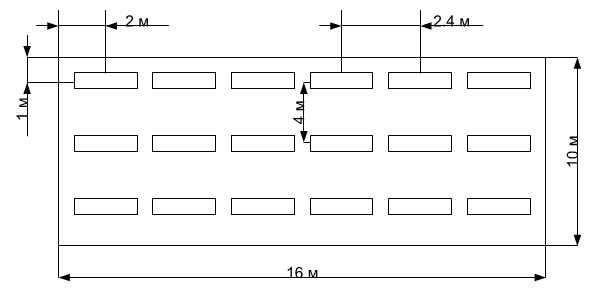
\includegraphics{static_include/illuminationScheme.png}
\caption{Схема освещения помещения}
\label{fig:illuminationScheme}
\end{figure}

При этом имеет место избыточное освещение, превышающее расчетный световой поток на $\frac{54-52}{52} = 3.8$\% (допустимым является 20\% отклонение).
Таким образом, в проекте используются 18 светильников с высотой подвеса 0.1 м и, соответственно, 54 люминесцентных ламп ЛБ-80 со световым потоком 5220 лм и световой отдачей 65.3 $\frac{\text{лм}}{\text{Вт}}$. Потребляемая мощность от светильников составляет 4320 Вт.
